% Short papers (up to 4 pages) and long papers (up to 10 pages). 
% All submissions must be single-spaced double-column pages using 10-point size font on 8.5x11 inch pages (IEEE conference style),
% including figures, tables, and references.
\documentclass[sigconf, anonymous, review,table]{acmart}
% The preceding line is only needed to identify funding in the first footnote. If that is unneeded, please comment it out.
\usepackage{hyperref}
\usepackage{amsmath,amsfonts}
\usepackage{algorithmic}
\usepackage{graphicx}
\usepackage{textcomp}
\usepackage{xcolor}
\usepackage{multirow}

\setcopyright{acmcopyright}
\copyrightyear{2018}
\acmYear{2018}
\acmDOI{XXXXXXX.XXXXXXX}

%% These commands are for a PROCEEDINGS abstract or paper.
\acmConference[Conference acronym 'XX]{Make sure to enter the correct
  conference title from your rights confirmation emai}{June 03--05,
  2018}{Woodstock, NY}
%%
%%  Uncomment \acmBooktitle if the title of the proceedings is different
%%  from ``Proceedings of ...''!
%%
%%\acmBooktitle{Woodstock '18: ACM Symposium on Neural Gaze Detection,
%%  June 03--05, 2018, Woodstock, NY}
\acmPrice{15.00}
\acmISBN{978-1-4503-XXXX-X/18/06}


%%
%% Submission ID.
%% Use this when submitting an article to a sponsored event. You'll
%% receive a unique submission ID from the organizers
%% of the event, and this ID should be used as the parameter to this command.
%%\acmSubmissionID{123-A56-BU3}

%%
%% For managing citations, it is recommended to use bibliography
%% files in BibTeX format.
%%
%% You can then either use BibTeX with the ACM-Reference-Format style,
%% or BibLaTeX with the acmnumeric or acmauthoryear sytles, that include
%% support for advanced citation of software artefact from the
%% biblatex-software package, also separately available on CTAN.
%%
%% Look at the sample-*-biblatex.tex files for templates showcasing
%% the biblatex styles.
%%

%%
%% The majority of ACM publications use numbered citations and
%% references.  The command \citestyle{authoryear} switches to the
%% "author year" style.
%%
%% If you are preparing content for an event
%% sponsored by ACM SIGGRAPH, you must use the "author year" style of
%% citations and references.
%% Uncommenting
%% the next command will enable that style.
%%\citestyle{acmauthoryear}


%%
%% end of the preamble, start of the body of the document source.
\begin{document}

%%
%% The "title" command has an optional parameter,
%% allowing the author to define a "short title" to be used in page headers.
\title[Generalized Sparse Linear Algebra Framework with Vendor-Agnostic GPUs Accelerated Computations]{Spla: Generalized Sparse Linear Algebra Framework with Vendor-Agnostic GPUs Accelerated Computations}

%%
%% The "author" command and its associated commands are used to define
%% the authors and their affiliations.
%% Of note is the shared affiliation of the first two authors, and the
%% "authornote" and "authornotemark" commands
%% used to denote shared contribution to the research.
\author{Egor Orachev}
\email{egor.orachev@gmail.com}
\orcid{0000-0002-0424-4059}
\author{Semyon Grigorev}
\email{s.v.grigoriev@spbu.ru}
\orcid{0000-0002-7966-0698}
\affiliation{%
  \institution{St. Petersburg State University}
  \streetaddress{7-9 Universitetskaya Embankmen}
  \city{St. Petersburg}  
  \country{Russia}
  \postcode{199034}
}



%%
%% By default, the full list of authors will be used in the page
%% headers. Often, this list is too long, and will overlap
%% other information printed in the page headers. This command allows
%% the author to define a more concise list
%% of authors' names for this purpose.
\renewcommand{\shortauthors}{Orachev, Grigorev}


\begin{abstract}
    Scalable high-performance graph analysis is an actual nontrivial challenge. Usage of sparse linear algebra operations as building blocks for graph analysis algorithms, which is a core idea of GraphBLAS standard, is a promising way to attack it.
    While it is known that sparse linear algebra operations can be efficiently implemented on GPU, full GraphBLAS implementation on GPU is a nontrivial task that is almost solved by GraphBLAST project. Though it is shown that utilization of GPUs for GraphBLAS implementation significantly improves performance, portability problem is not solved yet: GraphBLAST uses Nvidia Cuda stack. 
    Moreover, while GraphBLAS is stable and mature, it has some limitations discussed by John R. Gilbert at HPEC GraphBLAS BoF. 
    In this work we propose Spla library that aimed to solve some of these problems. The API of the library provides runtime information and introspection. Its implementation streamlines storage management, avoids implicit zeros and clarifies masking semantics, and provides GPUs accelerated computations.
    Evaluation shows that while further optimizations are required, the proposed solution demonstrates performance comparable with GraphBLAST, outperforming it up to 36 times in some cases, remaining portable across different GPUs vendors. Moreover, our solution on integrated GPU outperforms SuiteSparse:GrpaphBLAS on the respective CPU on some graph analysis tasks.
\end{abstract}

%%
%% The code below is generated by the tool at http://dl.acm.org/ccs.cfm.
%% Please copy and paste the code instead of the example below.
%%  
  
\begin{CCSXML}
<ccs2012>
 <concept>
   <concept_id>10002950.10003624.10003633.10010917</concept_id>
   <concept_desc>Mathematics of computing~Graph algorithms</concept_desc>
   <concept_significance>500</concept_significance>
 </concept>
 <concept>
   <concept_id>10010147.10010169.10010170</concept_id>
   <concept_desc>Computing methodologies~Parallel algorithms</concept_desc>
   <concept_significance>500</concept_significance>
 </concept>
 <concept>
   <concept_id>10010520.10010521.10010528.10010534</concept_id>
   <concept_desc>Computer systems organization~Single instruction, multiple data</concept_desc>
   <concept_significance>500</concept_significance>
 </concept>
</ccs2012>
\end{CCSXML}

\ccsdesc[500]{Mathematics of computing~Graph algorithms}
\ccsdesc[500]{Computing methodologies~Parallel algorithms}
\ccsdesc[500]{Computer systems organization~Single instruction, multiple data}

%%
%% Keywords. The author(s) should pick words that accurately describe
%% the work being presented. Separate the keywords with commas.
\keywords{graphs, algorithms, graph analysis, sparse linear algebra, GraphBLAS, GPGPU, OpenCL}

%%
%% This command processes the author and affiliation and title
%% information and builds the first part of the formatted document.
\maketitle


\section{Introduction}

Scalable high-performance graph analysis is an actual challenge.
There is a big number of ways to attack this challenge~\cite{Coimbra2021} and the first promising idea is to utilize general-purpose graphic processing units (GPGPU).
Such existing solutions, as CuSha~\cite{10.1145/2600212.2600227} and Gunrock~\cite{7967137} show that utilization of GPUs can improve the performance of graph analysis, moreover it is shown that solutions may be scaled to multi-GPU systems.
But low flexibility and high complexity of API are problems of these solutions.

The second promising thing which provides a user-friendly API for high-performance graph analysis algorithms creation is a GraphBLAS API~\cite{7761646} which provides linear algebra based building blocks to create graph analysis algorithms.
The idea of GraphBLAS is based on a well-known fact that linear algebra operations can be efficiently implemented on parallel hardware.
Along with that, a graph can be natively represented using matrices: adjacency matrix, incidence matrix, etc.
While reference CPU-based implementation of GraphBLAS, SuiteSparse~\cite{10.1145/3322125}, demonstrates good performance in real-world tasks, GPU-based implementation is challenging.

One of the challenges in this way is that real data are often sparse, thus underlying matrices and vectors are also sparse, and, as a result, classical dense data structures and respective algorithms are inefficient. 
So, it is necessary to use advanced data structures and procedures to implement sparse linear algebra, but the efficient implementation of them on GPU is hard due to the irregularity of workload and data access patterns.
Though such well-known libraries as cuSPARSE show that sparse linear algebra operations can be efficiently implemented for GPU, it is not so trivial to implement GraphBLAS on GPU. 
First of all, it requires \textit{generalized} sparse linear algebra, thus it is impossible just to reuse existing libraries which are almost all specified for operations over floats.
The second problem is specific optimizations, such as masking fusion, which can not be natively implemented on top of existing kernels.
Nevertheless, there is a number of implementations of GraphBLAS on GPU, such as GraphBLAST~\cite{yang2019graphblast}, GBTL~\cite{7529957}, which show that GPUs utilization can improve the performance of GraphBLAS-based graph analysis solutions.
But these solutions are not portable because they are based on Nvidia Cuda stack.

Although GraphBLAS is solid and mature standard with a number of implementation, it has limitations and shortcomings discussed in a talk given by John R. Gilbert~\cite{talk:graphblas_did_wrong}. Some of them are lack of interoperability and introspection, what is an obstacle on the way of GraphBLAS integration into real-world data analysis pipelines. Implicit zeroes mechanism and masking, which uses mix of engineering and math, leads to unpredictable memory usage in some cases, keeping API complex for both implementation and usage.

To provide portable linear algebra based GraphBLAS-inspired GPU graph analysis tool we developed a \textit{Spla} library\footnote{Source code of Spla library available at: \url{https://anonymous.link}}.
This library utilizes OpenCL for GPU computing to be portable across devices of different vendors and aimed to solve some of GraphBLAS limitations.
To sum up, the contribution of this work is the following.
\begin{itemize}
    \item Design of the library with GraphBLAS-inspired API proposed. The proposed solution addresses some GraphBLAS limitations, such as lack of introspection, implicit zeroes mechanism and ambiguous masking. Also, the core of the library is configurable, so GPU acceleration can be plugged in for some operations with a little effort.
    \item The proposed design implemented in C++ using OpenCL to provide GPU acceleration of some operations. Such linear algebra operations as matrix-vector multiplication for both dense and sparse vector, masked matrix-matrix multiplication, implemented on GPU. Totally, Spla provides all operations required to implement GPU-accelerated versions of breadth-first search (BFS), single source shortest path (SSSP), page rank (PR), and triangles counting (TC), that also are implemented.
    \item Evaluation on BFS, SSSP, PR, and TC, and real-world graphs shows portability across different vendors and promising performance: proposed solution consistently outperforms SuiteSparse, reaching up to 25 times speedup on some graphs, and shows performance comparable with GraphBLAST, achieving up to 36 times speedup in some cases. Surprisingly, for some problems, the proposed solution on integrated Intel GPU shows better performance than SuiteSparse on the respective CPU. At the same time, the evaluation shows that further optimizations are required.
\end{itemize}
\section{Background of Study}

This section provides a brief overview of existing solutions for graph analysis on both CPU and GPU, and also describes the concepts of the GraphBLAS standard, highlighting some of its shortcomings and limitations on the way to a full-fledged GPU implementation.

\subsection{Related Work}

There is a number of graph processing frameworks for a both CPU and GPU analysis. A greate survey of such frameworks is done by Batari et al.~\cite{article:batarfi_survey_graphs} and Shi et al.~\cite{article:shi_survey_graphs}. From an conceptual perspective, this frameworks can be roughly divided into three categories: vertex-centric, edge-centric, linear algebra-based.

\textit{Vertex-centric}. Introduces in Pregel~\cite{article:pregel} framework, vertex-centric model is based on a parallel processing of a graph vertices. The whole process is divided into iterations, where active vertices do a actual processing and send messages.  

\textit{Edge-centric}. Edge-centric model focuses on edges processing rather then vertices. It is first introduced in X-Stream~\cite{article:xstream} project. This model streams edges of the graphs and allows to effectively process them. 

\textit{Linear-algebra based}. Linear algebra based frameworks for a graph processing originate from a CombinationalBLAS~\cite{article:combblas} project. Linear algebra approach relies on the fact, that the graph traversal can be represented as matrix-vector multiplication. The graph analysis community has formalized this method in a GraphBLAS~\cite{7761646} standard, which provides linear algebra primitives in a form of C API. This standard has a number of implementations, including the reference implementation SuiteSparse~\cite{10.1145/3322125}, GBTL~\cite{7529957}, Huawei GraphBLAS implementation~\cite{article:hu_graphblas_impl}, GraphBLAST~\cite{yang2019graphblast}, etc.

\subsection{GraphBLAS concepts}

GraphBLAS standard~\cite{7761646} is a mathematical notation translated into a C API. This standard provides linear algebra building blocks for the implementation of graph algorithms in terms of operations over matrices and vectors. Essential parts of this standard are described below.

\textit{Data containers}. Primary data containers in this standard are general M by N matrix and M vector of values, as well as a scalar value. Containers are parameterised by the type of stored elements. As an example, matrix can be used to represent the adjacency matrix of the graph. Vector can be used to store a set of active vertices for traversal purposes. 

\textit{Algebraic structure}. Algebraic structures are called semiring and monoid, where two or one operation is provided respectively with some semantic requirements. These structures are adapted for containers, so their mathematical properties differ a bit from those, which are stated in classical algebra. These structures define the element-wise operations, which work with elements in vector and matrix containers. 

\textit{Operations.} GraphBLAS provides a number of commonly used linear algebra operations, such as \textit{mxv} and \textit{mxm}, element-wise multiplication, etc. Also, there are some extra operations, such as filtering, selection using predicate, reduction of matrix to vector or of vector to scalar, etc.

\textit{Programming constructs}. GraphBLAS provides extra objects, which are required for practical algorithms implementation, such a mask. Masking allows to use structure of matrix or vector to filter result and reduce amount of computations.

\textit{Algorithms.} Using GraphBLAS constructs it is possible with little effort to write generalized graph analysis algorithms, such as breadth-first search, single-source shortest path, triangles counting, connected components, etc.

\subsection{GraphBLAS limitations}

Although GraphBLAS is mature standard with a number of implementation, it has some limitations and shortcomings, discussed in a talk given by Gilbert~\cite{talk:graphblas_did_wrong}. Some of them are explained in the next paragraphs. 

\textit{C-oriented}. GraphBLAS standard is initially oriented on a C99 compatible API due to some technical and performance considerations. Standard does not considers any high-level built-in package for a more streamlined work with API.

\textit{Lack of interoperability}. GraphBLAS declares opaque objects with are hidden from the user structure. It is not possible to somehow extend or interact with an existing standard implementation. However, practical tasks may required integration of existing formats, storage into a library for practical analysis. 

\textit{Little introspection}. GraphBLAS declares a very limited functionality to inspect structure, state, type, behaviour, performance, correctness, progress of library primitives and operations. It is not feasible to build production-ready data-analysis platform without these features, which are common for all modern DBMS.

\textit{Implicit zeros}. GraphBLAS standard tries to use a mix of math and engineering concepts to address the values storage model. As the result, this model is to complex and not obvious for both mathematicians and programmers. Thus, inaccurate storage manipulations may cause a sufficient memory usage increase in your application even if you precisely follow the standard.

\textit{Masking}. GraphBLAS standard provides an ability to apply a mask to filter out result matrices or vectors. However, rules for selecting values from a mask are implicit and rely on selecting raw zero values, like in a C program. This mechanism is not configurable.

\textit{Templates usage}. There is a number of libraries which implement GraphBLAS in a form of C++ interface. These libraries heavily rely on a template meta programming for a generalization of a processed data. This approach simplifies implementation of the library. Auxiliary code is generated by the compiler. However, template-based approach requires the whole project recompilation for each executable and for any change of a user code.

\textit{GPU support}. GraphBLAS has no fully-featured implementation with GPU support. The primary reason for this is the complexity of the standard. There is a number of attempts to adopt GraphBLAS for a GPU analysis. But, most of them are focused only on Nvidia platform, what limits the portability of the potential solution.
\section{Proposed Solution Description}

This section describes the high-level details of the proposed solution. 
It highlights the design principles, high-level architecture of the solution, data storage representation, operations, and also shows differences from the GraphBLAS API.

\subsection{Design Principles}

Spla library is designed the way to maximize potential library performance, to simplify its implementation and extensions, and to provide the end-user verbose, but expressive interface allowing customization and precise control over operations execution. 
These ideas are captured in the following principles.

\begin{itemize}
    \item \textit{Optional acceleration}. Library is designed in a way, that GPU acceleration is fully plugable and optional part. Library can perform computations using standard CPU pipeline. If GPU acceleration is presented, library can offload a part of a work for it. It allows both non-trivial processing of the data on the CPU only, as well as possibility to integrate different backends in the future.  
    \item \textit{User-defined functions}. The user can create custom element-by-element functions to parameterize operations. Custom functions can be used for both CPU and GPU execution.
    \item \textit{Predefined scalar data types}. The library provides a set of built-in scalar data types that have a natural one-to-one relationship with native GPU built-in types. Data storage is transparent. The library interprets the data as POD-structures. The user can interpret individual elements as a sequence of bytes of a fixed size.
    \item \textit{Hybrid-storage format}. The library automates the process of data storage and preprocessing. It supports several data formats, chooses the best one depending on the situation.
    \item \textit{Exportable interface}. The library has a C++ interface with an automated reference-counting and with no-templates usage. It can be wrapped by C99 compatible API and exported to other languages, for example, in a form of a Python package.
\end{itemize}

\subsection{Architecture Overview}

The general idea of the proposed solution is depicted in Fig.~\ref{fig:design}. 
The core of the library and its main part is the CPU, which is the master node and controls all calculations. 
It is responsible for storing data, maintaining a registry with algorithms, and scheduling operations to perform. 
In this paradigm, the GPU is an optional backend for acceleration, implemented through a special interface. 
It can optionally store data in a specific format. 
The CPU can offload the calculation of a part of the operations to the GPU, if the corresponding operation is supported by the given accelerator.

The reason for this is that the CPU and GPU are inherently asymmetric in nature. 
The end-user uses CPU side API. Thus, some preprocessing on the CPU side must be always done in the majority of cases. In addition, access to data on the GPU and their storage is carried out differently due to the peculiarities of the execution of kernels. 
Also, VRAM is more expensive and has less capacity than RAM.
Therefore, RAM is a cache for VRAM, and data duplication can be neglected. 
In the end, the explicit separation of the CPU side from the GPU of the backend gives the modularity. 
This can be used not only to support different GPU technologies, but also to integrate multiple GPUs or distributed processing in the future.

\begin{figure}[t]
\centering
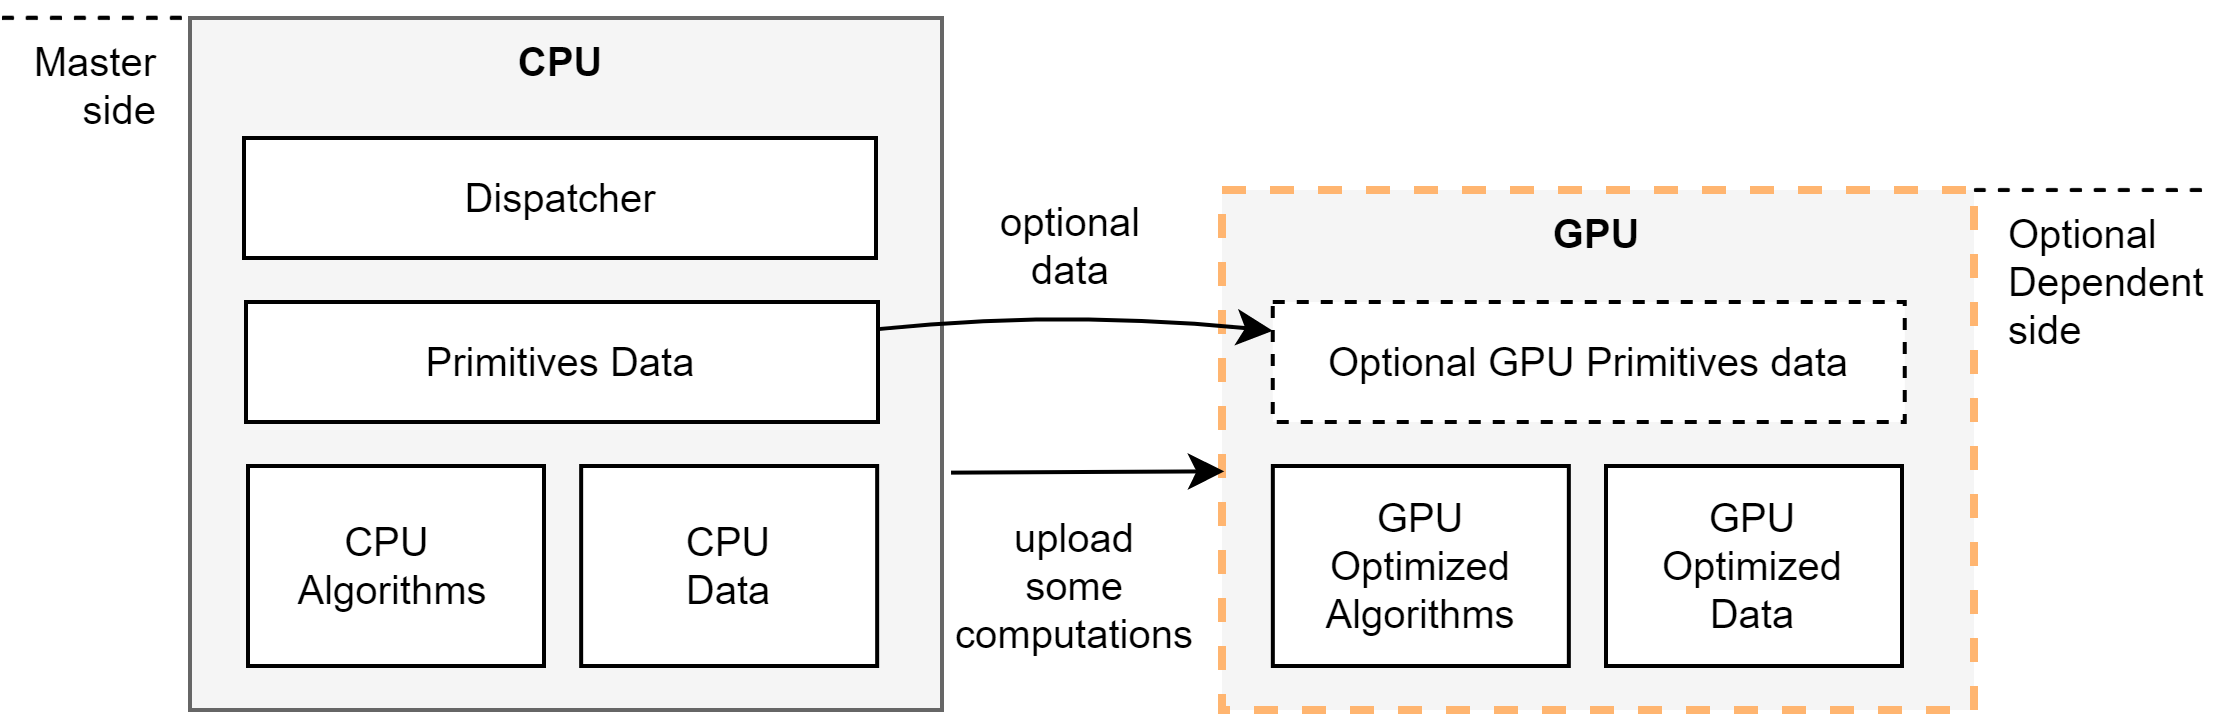
\includegraphics[width=0.95\linewidth]{figures/design_idea.png}
\caption{Proposed solution general design idea.}
\label{fig:design}
\end{figure}
    
\subsection{Data Containers}

Library provides general \textit{M-by-N Matrix}, \textit{N Vector} and \textit{Scalar} data containers.
Underlying primitive scalar types are specified by \textit{Type} object. 
Single vector or matrix data is stored in specialized multi-format storage container. An example of the single vector storage is depicted in Fig.~\ref{fig:vec_storage}. 

The storage is responsible for keeping data in multiple different formats at the same time. 
Each format is best suited for a specific type of task and requested on demand. 
Key-value dictionary suites well frequent insertion, query or deletion operations, when memory usage and response time are critical. 
Mathematical operations perform better with compacted sequential lists of values since they have more friendly cache behaviour. 
GPU operations require separate format with a copy of the data resident in VRAM.

Data transformation from one format to another is carried out using a special rules graph shown in Fig.~\ref{fig:vec_tsf}. 
The directed edges in this graph indicate conversion rules. 
The graph must be the single strongly connected component. 
An example of the data transformation process is depicted in Fig.~\ref{fig:vec_exmp}. 
For a requested format the best path of convertation is obtained. Currently, the shortest one is used. 
Weight assignment to rules can potentially be used to prioritize convertations and reduce the cost of transformation for some formats. 

Currently, several storage formats are supported. 
There is dictionary of keys for vector and matrix (DoK), list of coordinates (COO), dense vector, list of lists (LIL) and compressed sparse rows (CSR) matrix formats.  
Other formats, such as CSC, DCSR, ELL, etc., can be added to the library by the implementation of formats conversion and by the specialization of operations for a specific format.

\begin{figure}[b]
\centering
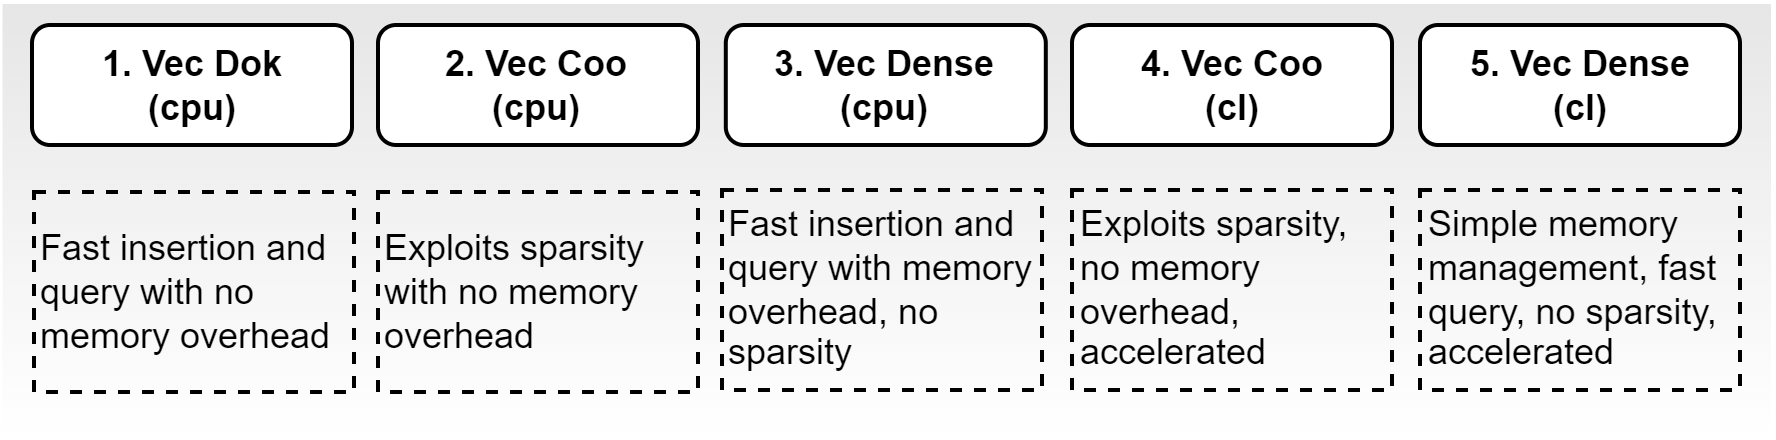
\includegraphics[width=0.9\linewidth]{figures/vector_storage.png}
\caption{Vector primitive storage holds the same data potentially in multiple different formats. Some slots can be empty.}
\label{fig:vec_storage}
\end{figure}

\begin{figure}[]
\centering
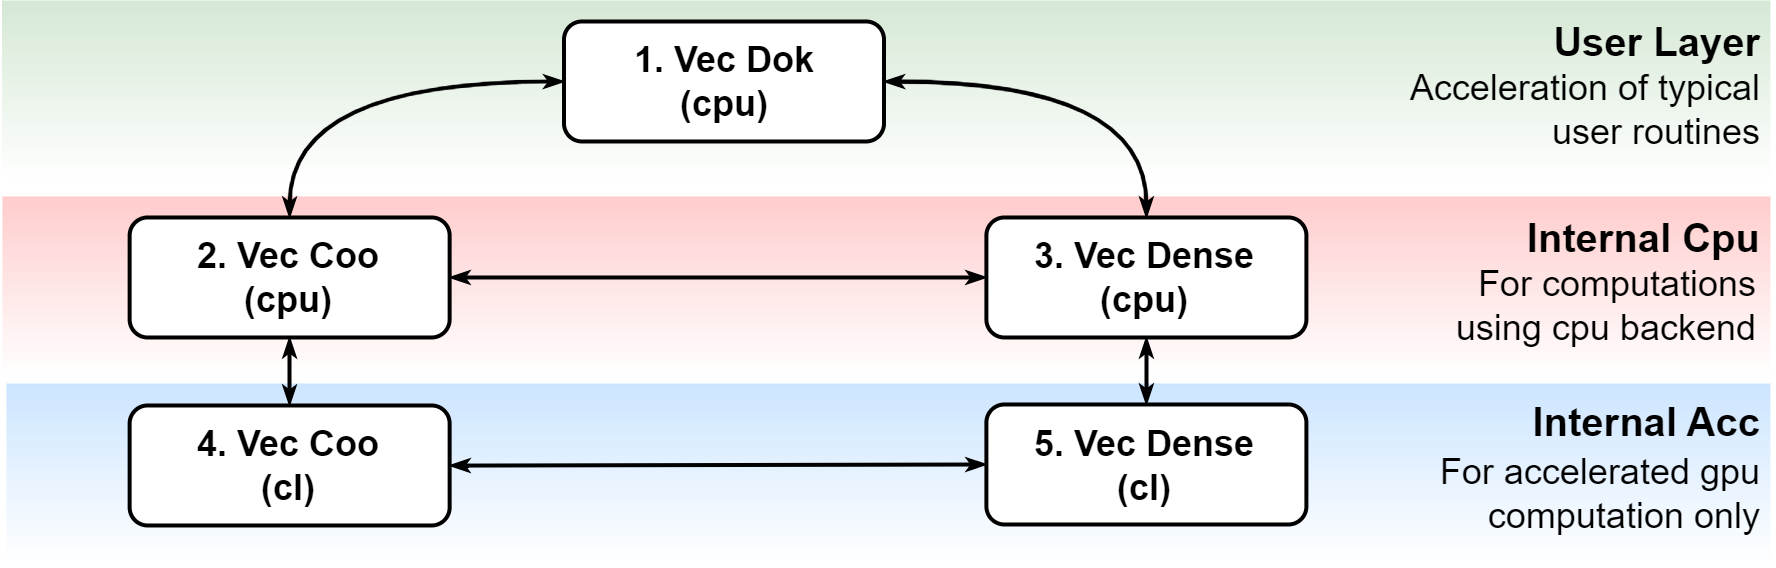
\includegraphics[width=0.9\linewidth]{figures/storage_transformation_graph.png}
\caption{Vector storage transformation graph. The graph defines how data can be obtained from one format in another.}
\label{fig:vec_tsf}
\end{figure}

\begin{figure}[]
\centering
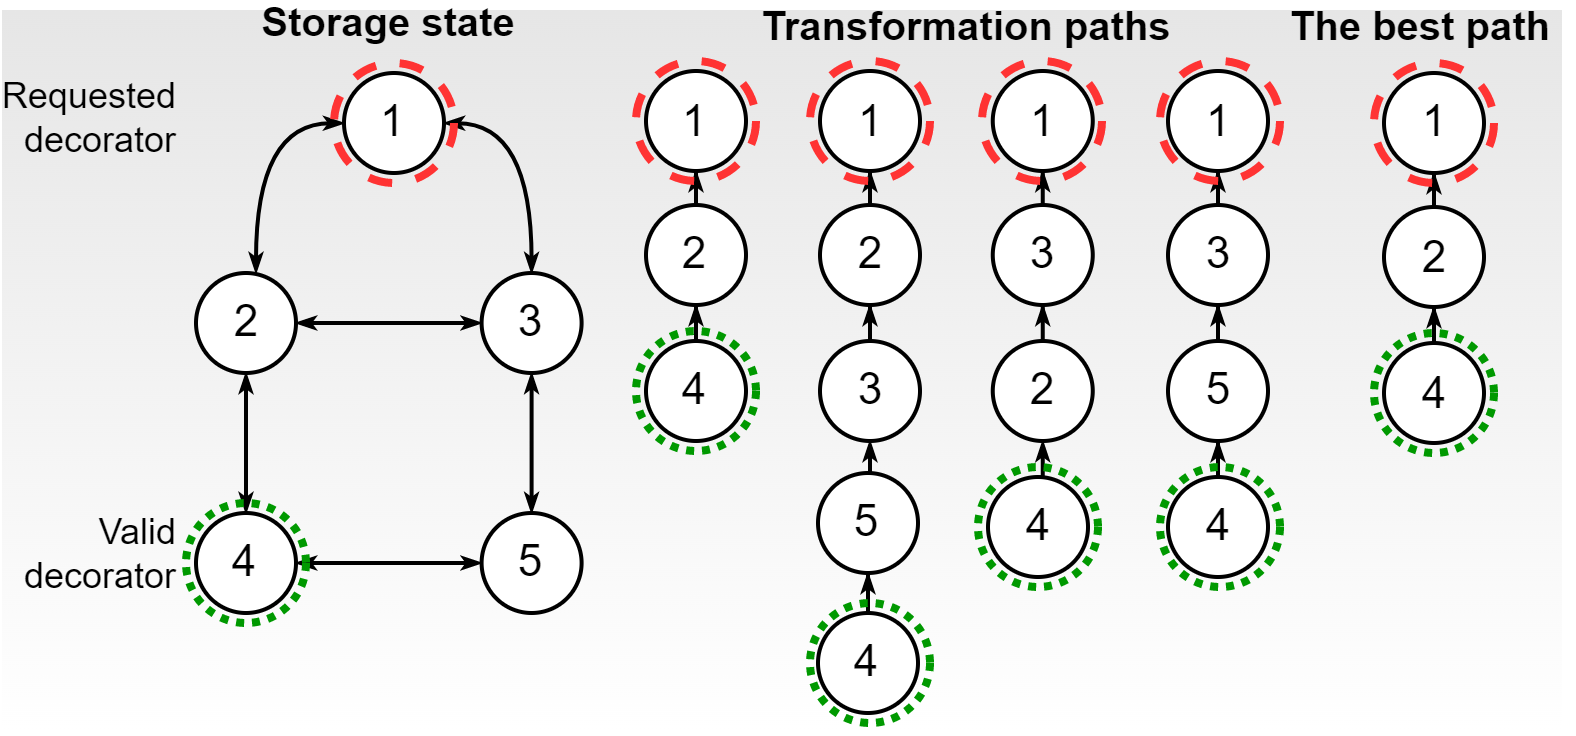
\includegraphics[width=0.9\linewidth]{figures/storage_transformation.png}
\caption{Vector storage transformation process. Green is valid format. Red is requested format. No highlight is currently invalid format.}
\label{fig:vec_exmp}
\end{figure}

\subsection{Algebraic Operations}

Library provides a number of commonly used operations, such as \textit{vxm}, \textit{mxv}, \textit{mxmT}, \textit{element-wise add}, \textit{assign}, \textit{map}, \textit{reduce}, etc.
Other operations can be added on demand.
Interface of operations is inspired by GraphBLAS standard. 
It supports \textit{masking}, parametrization by \textit{binary mult} and \textit{binary add} functions, \textit{select} for filtering and mask application, \textit{unary op} for values transformation, and \textit{descriptor} object for additional operation tweaking.

\subsection{Differences with GraphBLAS standard}

To be clear, the proposed solution is not an implementation of GraphBLAS C or C++ API. 
The design of the library uses only the concepts described in the standard. 
However, in the proposed solution, the signatures and semantics of some of the operations have been changed. 
The API has been made more verbose and explicit. 
In particular, the handling of \textit{zero} elements and \textit{masking} are made cleaner for the end user. The library interprets data simply as collections of bytes, without mathematical semantics and identity elements.
Identity element must be explicitly passed by the user where required. It allows to make the memory usage predictable and the result of each operation clear to the end user without internal implicit storage manipulations.
\section{Implementation Details}

This section describes implementation details of the proposed solution. 
It highlights key aspects of the core implementation, OpenCL specifics, optimization of particular operations, and high-level optimizations of graph algorithms.

\subsection{Core}

The implemented library uses the concept of a registry to find operations as shown in Fig.\ref{fig:reg}. A call to a particular operation is stored as a command to be executed later by \textit{Dispatcher}. For each command the special lightweight string key is built depending on type of the operation and arguments passed. This key is used as a regex to get the required implementation of the requested operation. The advantages of the proposed approach are listed below.

\begin{itemize}
    \item \textit{Late binding}. The operation call becomes a command. The processing of such a command can be configured at run time. Changing the acceleration backend can be done without recompilation. Moreover, several backends can be transparently used within a single application.
    \item \textit{Optionality of accelerator}. The acceleration backend is free to support only those operations that require it. Fallback implementations will be used automatically for the rest of the operations.
    \item \textit{Performance tuning}. The key of the command reflects operation type, arguments types, passed user functions types, etc. It can be used for \textit{ad-hoc} optimizations. Custom operation implementation with a verbose key can be also stored in the registry. If several operations match the key, the longest key is used, since it is more specific for a particular operation.
    \item \textit{Scheduling}. The full list of submitted commands for execution can be examined at runtime. This opens up the possibility for the fusion of some operations, sorting, rearrangement, and any other high-level optimizations that require introspection.
\end{itemize}

\begin{figure}[]
\centering
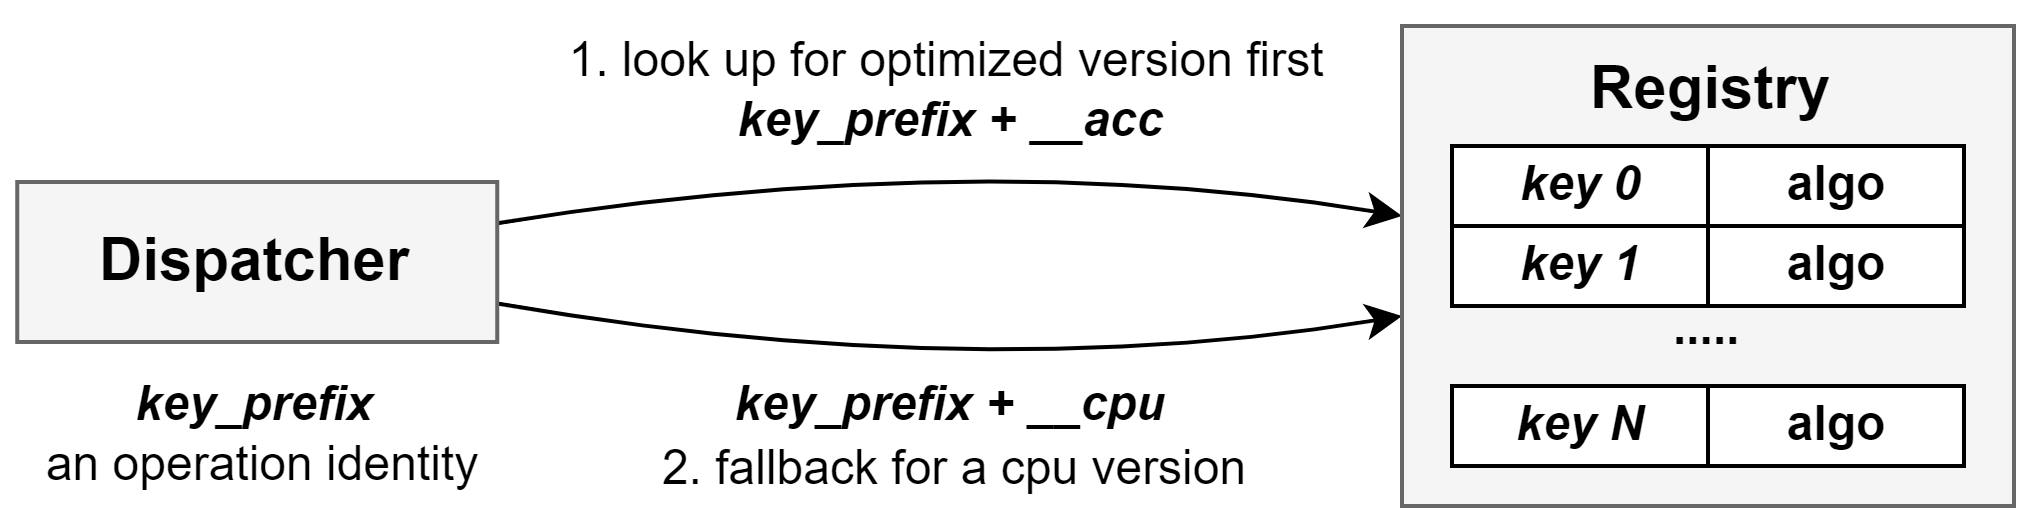
\includegraphics[width=0.95\linewidth]{figures/registry.png}
\caption{Registry of operation implementations. Keys with special syntax used to fetch required operation in a specific order at runtime.}
\label{fig:reg}
\end{figure}

\subsection{OpenCL}

OpenCL 1.2 is used as the primary API for backend GPU implementation. Header files with C and C++ definitions are supplied with the source code of the project. Official Khronos installable client driver (ICD) loader bundled within a library to load at runtime particular OpenCL implementation depending on running OS and GPU vendor. 

Implementation of sparse linear algebra algorithms for a GPU requires auxiliary libraries for memory management, sorting, reducing, merging, scanning, etc. 
Nvidia Cuda platform features libraries such as Thrust and Cub.  
OpenCL lacks such support. All primitives must be implement from a scratch in most cases. What is an extra challenge. Third-party library, such as Boost Compute~\cite{10.1145/2909437.2909454:boost:compute}, cannot be used, since it has significant runtime overhead, portability and performance issues, and lack of long term support.

User-defined functions for GPU usage are represented as strings with additional metadata, such as type of parameters, return types, unique id, etc. 
Source code of particular operations stored in a form of .cl files. 
Operations implemented with generalization for parameters types and user functions. 
Their definitions obtained later at runtime in a compilation step through the text pre-processing.
Compilation of actual OpenCL kernels is done on demand. 
All compiled kernels are stored in a cache. Cache key is composed from types of kernel parameters, defines, etc., which identify uniquely a particular variation of a kernel. 
Key composition is done in O(1). In-place allocation is utilized for a key builder to avoid global heap usage. 
In order to reduce CPU overhead and keep access to the cache fast, library uses robin hood hashing based hash map. 

Custom linear memory allocator implemented in order to reduce the overhead of frequent and small buffer allocations, arising in a time of execution of some operations. Allocator uses sub-buffer mechanism and serves request typically less than 1 MB of size. Otherwise, the general GPU heap is used.

\subsection{Linear Algebra Operations}

The following primitives are the core of computations: \textit{masked sparse-vector sparse-matrix product}, \textit{masked sparse-matrix dense-vector product} and \textit{masked sparse-matrix sparse-matrix product}. Efficient implementation and load balancing of those operations dominate the performance of particular algorithms. The following paragraphs give an insight into these operations implementation in the library.

\textit{Masked sparse-vector sparse-matrix product}. The implementation is based on the algorithm proposed by Yang et al.~\cite{7284398:spvspm}. It is a \textit{k}-way merge based algorithm which suites well for sparse vectors. Our implementation uses custom gather to collect temporary products. Radix sort used to sort products for further reduction. Reduction by key uses parallel prefix scan to carry out final destination of reduced values.

\textit{Masked sparse-matrix dense-vector product}. The implementation of this operation relies on a classic row-based parallel algorithm. Both scalar and vector versions are implemented to fit better relatively sparse and dense matrix rows. 

\textit{Masked sparse-matrix sparse-matrix product}. The implementation of this algorithm uses the approach proposed by Yang et al.~\cite{yang2019graphblast}. It is straightforward single-pass row-major and column-major matrix product. Mask is used to estimate the size of the final result to filter out some result of the product. 

\subsection{Graph Algorithms}

The advantage of the linear algebra approach is that graph algorithms can be easily composed of primitive operations using a few lines of code. For preliminary study breadth-first search (BFS), single-source shortest paths (SSSP), page rank (PR) and triangles counting (TC) algorithms were chosen. These are the most commonly evaluated graph algorithms. They allow to test basic operations and key aspects of graph frameworks performance. Implementation details for chosen algorithms are given below. 

\textit{BFS}. It utilizes a number of optimizations described by Yang et al.~\cite{https://doi.org/10.48550/arxiv.1804.03327:pushpull}. It uses masking to filter out already reached vertices, change of direction (push-pull) to switch from sparse from to dense and vice versa, and early exit in \textit{mxv} operation.

\textit{SSSP}. This algorithm uses change of direction as well. Also, it employs filtering of unproductive vertices according to Yang et al.~\cite{yang2019graphblast}. Vertices which do not relax their distance in current iteration are removed from a front of the search. It allows to keep workload moderate. 

\textit{PR}. This algorithm assigns numerical weights to objects in the network depending on their relative relevance. As a key operation it uses \textit{mxv} operation with a dense vector. For error estimation it uses custom element-wise function with a fusion of subtraction and square operations.  

\textit{TC}. Triangles counting uses masked sparse matrix product~\cite{yang2019graphblast} and reduction. As an input algorithm accepts a lower triangular component $L$ of an adjacency matrix of the source graph. The result is a count of non-zero values from $B = LL^T .* L$, where $.*$ used for the masking. The second argument is not actually transposed, since row-column based product gives exactly the required effect.
\section{Evaluation}

While our project\footnote{GraphBLAS\# project page: \url{https://github.com/YaccConstructor/GraphBLAS-sharp}.} is in a very early stage we implemented and evaluated only generic matrix-matrix element-wise function \texttt{map2} to demonstrate that the proposed solution may provide not only a way to an expressive compact high-level API, but also a way to its high-performance implementation. This function implemented for matrices in CSR format. We use Brahma.FSharp to support GPGPUs.  

We evaluate \texttt{map2} function parameterized by two operations: \texttt{op\_int\_add} (listing~\ref{lst:opIntAdd}) to get element-wise addition in terms of GraphBLAS API, and \texttt{op\_int\_mult} (listing~\ref{lst:opIntMult}) to get element-wise multiplication.

\subsection{Environment}
We perform our experiments on the PC with Ubuntu 20.04 installed and with the following hardware configuration: Intel Core i7--4790 CPU, 3.60GHz, 32GB DDR4 RAM with GeForce GTX 2070, 8GB GDDR6, 1.41GHz.

For comparison we choose a SuiteSparse:GraphBLAS as a reference CPU implementation of GraphBLAS API, and CUSP\footnote{Cusp is a CUDA-based library for sparse linear algebra and graph computations: \url{https://cusplibrary.github.io/}.} as a most stable GPGPU implementation of generic sparse linear algebra.

\begin{table}[H]
    \centering
    \caption{Matrices for evaluation}
    \label{matrices}  
    \begin{tabular}{ | c || c | c | c | }
    \hline
    Matrix & Size & NNZ & Squared matrix NNZ \\ \hline
    \hline
    wing & 62 032 & 243 088 & 714,200 \\ \hline
    luxembourg\_osm & 114 599 & 119 666 & 393 261 \\ \hline
    amazon0312 & 400 727 & 3 200 440 & 14 390 544 \\ \hline
    amazon-2008 & 735 323 & 5 158 388 & 25 366 745 \\ \hline
    web-Google & 916 428 & 5 105 039 & 29 710 164 \\ \hline
    webbase-1M & 1 000 005 & 3 105 536 & 51 111 996 \\ \hline
    cit-Patents & 3 774 768 & 16 518 948 & 469 \\ \hline
    \end{tabular}
\end{table}


\subsection {Dataset}

For evaluation we select a set of matrices from SuiteSparse matrix collection\footnote{SuiteSparse matrix collection: \url{https://sparse.tamu.edu/}.}
To simplify the evaluation of element-wise operations over matrices with different structures we precomputed the square of each matrix.
Characteristics of selected matrices are presented in table~\ref{matrices}.

\subsection{Evaluation Results}

\begin{table*}[h]
    \centering    
    \caption{Evaluation results for element-wise operations, time in ms}    
    \label{perf-comparison}
    \begin{tabular}{|c||c|c|c|c||c|c|}
    \hline
    \multirow{3}{*}{Matrix} & \multicolumn{4}{c||}{Elemint-wise addition} & \multicolumn{2}{c|}{Elemint-wise multiplication}\\    
    \cline{2-7}        
    & \multicolumn{2}{c|}{GraphBLAS-sharp} & \multirow{2}{*}{SuiteSparse} & \multirow{2}{*}{CUSP} & \multirow{2}{*}{GraphBLAS-sharp} & \multirow{2}{*}{SuiteSparse}        \\
    &No \texttt{AtLeastOne}&\texttt{AtLeastOne}& & & &\\ 
    \hline
    \hline
    wing            & $4,3 \pm 0,8$       & $4,3 \pm 0,6$      & $2,7\pm 0,9$   & $1,5\pm 0,0$   & $3,7 \pm 0,5$      & $3,5\pm 0,4$\\
    \hline
    luxembourg\_osm & $4,9 \pm 0,7$       & $4,1 \pm 0,5$      & $3,0\pm 1,1$   & $1,2\pm 0,1$  & $3,8 \pm 0,6$      & $3,0\pm 0,6$ \\
    \hline
    amazon0312      & $22,3 \pm 1,3$       & $22,1 \pm 1,3$      & $33,4\pm 0,8$  & $11,0\pm 1,4$  & $18,7 \pm 0,9$      & $35,7\pm 1,4$ \\
    \hline
    amazon-2008     & $38,7 \pm 0,8$       & $39,0 \pm 1,0$     & $55,9\pm 1,0$  & $19,1\pm 1,4$ & $34,5 \pm 1,0$     & $58,9\pm 1,9$  \\
    \hline
    web-Google      & $43,4 \pm 0,8$       & $43,4 \pm 1,1$     & $67,2\pm 7,5$  & $21,3\pm 1,3$  & $39,0 \pm 1,2$     & $66,2\pm 0,4$ \\
    \hline
    webbase-1M      & $63,6 \pm 1,1$      & $63,7 \pm 1,3$      & $86,5\pm 2,0$  & $24,3\pm 1,3$  & $54,5 \pm 0,7$      & $37,6\pm 5,6$ \\
    \hline
    cit-Patents     & $26,9 \pm 0,7$      & $26,0 \pm 0,7$      & $183,4\pm 5,4$ & $10,8\pm 0,6$   & $24,3 \pm 0,7$      & $162,2\pm 1,7$ \\     
    \hline
    \end{tabular}    
\end{table*}

To benchmark .NET-based implementation we use \textit{BenchmarkDotNet}\footnote{\textit{BenchmarkDotNet}: \url{https://benchmarkdotnet.org/}. Access date: 12.06.2022.} which allows one to automate benchmarking process for .NET platform.
We run each function XXX times, !!!
Time is measured in milliseconds. The time to prepare data and initially transfer it to GPU is not included.

Results of performance evaluation are presented in table~\ref{perf-comparison}.
We can see, that for element-wise addition our implementation slightly slower than SuiteSparse:GraphBLAS for small matrices (\textbf{wing, luxembourg\_osm}) and up to 7 times faster for big matrices (1.5 times median). At the same time our implementation 2.5 times slower than CUSP-based. For element-wise multiplication comparison with SuiteSparse:GraphBLAS shows almost similar results except matrix \textbf{webbase-1M} for which our implementation slower than SuiteSparse:GraphBLAS.

Comparison between original element-wise addition over primitive types, without \texttt{AtLeasOne} and generalized version which uses \texttt{AtLeastOne} type is also presented in table~\ref{perf-comparison}.
We can see, that more complex data types and element-wise operations do not poor performance of matrix-matrix operations because data transfer dominates arithmetic computations for sparse matrices processing, and the proposed abstraction does not increase the memory footprint.

\section{Conclusion}

We presented Spla, generalized sparse linear algebra framework with vendor-agnostic GPUs accelerated computations. Library design addresses some GraphBLAS limitations, such as lack of interoperability, implicit zeroes and inflexible masking. The evaluation of the proposed solutions for some real-world graph data in four different algorithms shows, that OpenCL-based solution has a promising performance, comparable to analogs, has acceptable scalability on devices of different GPU vendors, and, surprisingly, has a speedup in some cases when compared with highly-optimized CPU library on some integrated GPUs. All in all, there are still a plenty of research questions and directions for improvement. Some of them are listed bellow.

\begin{itemize}
    \item \textit{Performance tuning}. There is a still space for optimizations. Better workload balancing must be done. Performance must be improved on AMD and Intel devices. More optimized algorithms must be implemented, such as SpGEMM  algorithm proposed by Nagasaka et al.~\cite{8025284/spgemm/nagasaka} for general \textit{mxm} operation.
    \item \textit{Operations}. Additional linear algebra operations must be implemented as well as useful subroutines for filtering, joining, loading, saving data, and other manipulations involved in typical graphs analysis.
    \item \textit{Graph streaming}. The next important direction of the study is streaming of data from CPU to GPU. CuSha adopt data partitioning techniques for graphs processing which do not fit single GPU. Modern GPUs have a limited VRAM. Even high-end devices allow only a moderate portion of the memory to be addressed by the kernel at the same time. Thus, manual streaming of the data from CPU to GPU is required in order to support analysis of extremely large graphs, which count billions of edges to process.
    \item \textit{Multi-GPU}. Finally, scaling of the library to multiple GPUs must be implemented. Gunrock shows, that such approach can increase overall throughput and speedup processing of really dense graph. In connection with a streaming, it can be an ultimate solution for a large real-world graphs analysis.
\end{itemize}

\bibliographystyle{ACM-Reference-Format}
\bibliography{spla_main}

\appendix
\section{Detailed Evaluation Results}

Evaluation results TODO

\begin{table}[tbp]
    \caption{Performance comparison of the proposed solution.\\Time in milliseconds (lower is better).} 
    \begin{center}
        \begin{tabular}{|l|r|r|r|r|}
        \hline
        Dataset & GB & GR & LG & SP \\
        \hline
        \hline
        \multicolumn{5}{|c|}{BFS} \\
        \hline
        \rowcolor{black!10} coAuthorsCit&5.0&1.9&6.3&6.9\\
        \rowcolor{black!2 } coPapersDBLP&19.9&4.5&18.0&11.5\\
        \rowcolor{black!10} amazon2008&8.3&3.3&20.4&8.1\\
        \rowcolor{black!2 } hollywood2009&64.3&20.3&23.4&20.3\\
        \rowcolor{black!10} belgiumosm&200.6&84.4&138.0&181.2\\
        \rowcolor{black!2 } roadNetCA&116.3&32.4&168.2&101.7\\
        \rowcolor{black!10} comOrkut& none&205.0&40.6&53.2\\
        \rowcolor{black!2 } citPatents&30.6&41.3&115.9&35.1\\
        \rowcolor{black!10} rggn222s0&367.3&95.9&1228.1&415.3\\
        \rowcolor{black!2 } socLiveJournal&63.1&61.0&75.5&57.1\\
        \rowcolor{black!10} indochina2004& none&33.3&224.6&328.7\\
        \rowcolor{black!2 } rggn223s0&615.3&146.2&2790.0&754.9\\
        \rowcolor{black!10} roadcentral&1383.4&243.8&1951.0&710.2\\
        \hline
        \hline
        \multicolumn{5}{|c|}{SSSP} \\
        \hline
        \rowcolor{black!10} coAuthorsCit&14.7&2.1&38.9&10.3\\
        \rowcolor{black!2 } coPapersDBLP&118.6&5.6&92.2&25.7\\
        \rowcolor{black!10} amazon2008&43.4&4.0&90.0&21.7\\
        \rowcolor{black!2 } hollywood2009&404.3&24.6&227.7&57.5\\
        \rowcolor{black!10} belgiumosm&650.2&81.1&1359.8&240.9\\
        \rowcolor{black!2 } roadNetCA&509.7&32.4&1149.3&147.9\\
        \rowcolor{black!10} comOrkut& none&219.0&806.5&241.0\\
        \rowcolor{black!2 } citPatents&226.9&49.8&468.5&129.3\\
        \rowcolor{black!10} rggn222s0&21737.8&101.9&4808.8&865.4\\
        \rowcolor{black!2 } socLiveJournal&346.4&69.2&518.0&189.5\\
        \rowcolor{black!10} indochina2004& none&40.8&821.9&596.6\\
        \rowcolor{black!2 } rggn223s0&59015.7&161.1&11149.9&1654.8\\
        \rowcolor{black!10} roadcentral&13724.8&267.0&25703.4&1094.3\\
        \hline
        \hline
        \multicolumn{5}{|c|}{PR} \\
        \hline
        \rowcolor{black!10} coAuthorsCit&1.6&10.0&24.3&3.2\\
        \rowcolor{black!2 } coPapersDBLP&17.6&120.2&297.6&6.1\\
        \rowcolor{black!10} amazon2008&5.2&40.6&89.8&5.5\\
        \rowcolor{black!2 } hollywood2009&62.9&559.5&1111.2&32.4\\
        \rowcolor{black!10} belgiumosm&4.4&22.9&167.6&9.4\\
        \rowcolor{black!2 } roadNetCA&6.6&37.7&225.8&19.6\\
        \rowcolor{black!10} comOrkut& none&2333.6&5239.0&103.3\\
        \rowcolor{black!2 } citPatents&27.0&686.1&1487.0&38.3\\
        \rowcolor{black!10} rggn222s0&45.2&320.0&563.5&26.6\\
        \rowcolor{black!2 } socLiveJournal& none&445.9&2122.5&112.0\\
        \rowcolor{black!10} rggn223s0& none&662.7&1155.6&103.4\\
        \rowcolor{black!2 } roadcentral& none&408.8&2899.9&172.0\\
        \hline
        \hline
        \multicolumn{5}{|c|}{TC} \\
        \hline
        \rowcolor{black!10} coAuthorsCit&2.3&2.0&17.3&3.0\\
        \rowcolor{black!2 } coPapersDBLP&105.2&5.3&520.8&128.4\\
        \rowcolor{black!10} amazon2008&11.2&3.9&73.9&10.8\\
        \rowcolor{black!2 } roadNetCA&6.5&32.4&46.0&7.7\\
        \rowcolor{black!10} comOrkut&1776.9&218.0&23103.8&2522.0\\
        \rowcolor{black!2 } citPatents&65.5&49.7&675.0&54.5\\
        \rowcolor{black!10} socLiveJournal&504.3&69.2&3886.7&437.8\\
        \rowcolor{black!2 } rggn222s0&73.2&101.3&484.5&77.7\\
        \rowcolor{black!10} rggn223s0&151.4&158.9&1040.1&204.2\\
        \rowcolor{black!2 } roadcentral&42.6&259.3&425.3&52.7\\
        \hline
        \hline
        \multicolumn{5}{l}{GraphBLAST (GB), Gunrock (GR), LaGraph (LG), Spla (SP).} \\
        \end{tabular}
        \label{rq1_table}
    \end{center}
    \end{table}
    
    \begin{table}[tbp]
    \caption{Portability of the proposed solution.\\Time in milliseconds (lower is better).} 
    \begin{center}
        \begin{tabular}{|l|r|r|r|}
        \hline
        Dataset & Intel Arc & AMD Vega & Nvidia Gtx\\
        \hline
        \hline
        \multicolumn{4}{|c|}{BFS} \\
        \hline
        \rowcolor{black!10} coAuthorsCit&12.8&8.3&6.9\\
        \rowcolor{black!2 } coPapersDBLP&10.8&14.9&11.5\\
        \rowcolor{black!10} amazon2008&12.3&12.6&8.1\\
        \rowcolor{black!2 } hollywood2009&15.3&26.7&20.3\\
        \rowcolor{black!10} belgiumosm&627.5&292.4&181.2\\
        \rowcolor{black!2 } roadNetCA&265.5&259.8&101.7\\
        \rowcolor{black!10} comOrkut&33.2&63.6&53.2\\
        \rowcolor{black!2 } citPatents&21.0&30.3&35.1\\
        \rowcolor{black!10} rggn222s0&825.3&1259.7&415.3\\
        \rowcolor{black!2 } socLiveJournal&43.0&85.8&57.1\\
        \rowcolor{black!10} indochina2004&220.6&573.4&328.7\\
        \rowcolor{black!2 } rggn223s0&1245.5&2519.6&754.9\\
        \rowcolor{black!10} roadcentral&1864.9&1680.8&710.2\\
        \hline
        \hline
        \multicolumn{4}{|c|}{SSSP} \\
        \hline
        \rowcolor{black!10} coAuthorsCit&18.3&10.4&10.3\\
        \rowcolor{black!2 } coPapersDBLP&22.9&27.7&25.7\\
        \rowcolor{black!10} amazon2008&23.4&22.2&21.7\\
        \rowcolor{black!2 } hollywood2009&44.6&56.2&57.5\\
        \rowcolor{black!10} belgiumosm&1085.9&454.8&240.9\\
        \rowcolor{black!2 } roadNetCA&447.3&422.5&147.9\\
        \rowcolor{black!10} comOrkut&79.7&111.5&241.0\\
        \rowcolor{black!2 } citPatents&49.8&78.4&129.3\\
        \rowcolor{black!10} rggn222s0&1378.8&924.3&865.4\\
        \rowcolor{black!2 } socLiveJournal&82.7&120.7&189.5\\
        \rowcolor{black!10} indochina2004&366.2&519.0&596.6\\
        \rowcolor{black!2 } rggn223s0&1880.2&1201.4&1654.8\\
        \rowcolor{black!10} roadcentral&3176.3&2848.8&1094.3\\
        \hline
        \hline
        \multicolumn{4}{|c|}{PR} \\
        \hline
        \rowcolor{black!10} coAuthorsCit&3.9&1.0&3.2\\
        \rowcolor{black!2 } coPapersDBLP&5.7&6.1&6.1\\
        \rowcolor{black!10} amazon2008&25.2&4.0&5.5\\
        \rowcolor{black!2 } hollywood2009&22.6&32.4&32.4\\
        \rowcolor{black!10} belgiumosm&10.2&7.1&9.4\\
        \rowcolor{black!2 } roadNetCA&10.8&15.7&19.6\\
        \rowcolor{black!10} comOrkut&31.9&46.6&103.3\\
        \rowcolor{black!2 } citPatents&12.3&21.3&38.3\\
        \rowcolor{black!10} rggn222s0&13.4&22.4&26.6\\
        \rowcolor{black!2 } socLiveJournal&210.0&64.2&112.0\\
        \rowcolor{black!10} rggn223s0&38.6&57.2&103.4\\
        \rowcolor{black!2 } roadcentral&57.9&89.6&172.0\\
        \hline
        \hline
        \multicolumn{4}{|c|}{TC} \\
        \hline
        \rowcolor{black!10} coAuthorsCit&4.6&2.2&3.0\\
        \rowcolor{black!2 } coPapersDBLP&57.6&106.2&128.4\\
        \rowcolor{black!10} amazon2008&6.9&8.5&10.8\\
        \rowcolor{black!2 } roadNetCA&5.4&5.4&7.7\\
        \rowcolor{black!10} comOrkut&1533.5&3267.6&2522.0\\
        \rowcolor{black!2 } citPatents&25.9&39.8&54.5\\
        \rowcolor{black!10} socLiveJournal&280.6&420.3&437.8\\
        \rowcolor{black!2 } rggn222s0&21.0&57.8&77.7\\
        \rowcolor{black!10} rggn223s0&56.7&123.2&204.2\\
        \rowcolor{black!2 } roadcentral&14.5&34.6&52.7\\
        \hline
        \hline
        \multicolumn{4}{l}{Distinct devices. Performance in not for comparison.} \\
        \end{tabular}
        \label{rq2_table}
    \end{center}
    \end{table}
    
    \begin{table}[tbp]
    \caption{Integrated GPU mode performance comparison of the proposed solution. Time in milliseconds (lower is better).} 
    \begin{center}
        \begin{tabular}{|l|r|r|r|r|}
        \hline
        \multirow{2}{*}{Dataset} & \multicolumn{2}{c|}{Intel} & \multicolumn{2}{c|}{AMD} \\
        \cline{2-5}
        & LG & SP & LG & SP \\
        \hline
        \hline
        \multicolumn{5}{|c|}{BFS} \\
        \hline
        \rowcolor{black!10} coAuthorsCit&7.5&26.3&3.9&18.2\\
        \rowcolor{black!2 } coPapersDBLP&18.7&57.3&12.0&54.9\\
        \rowcolor{black!10} amazon2008&24.6&65.0&13.5&40.0\\
        \rowcolor{black!2 } hollywood2009&23.8&100.1&14.8&86.6\\
        \rowcolor{black!10} belgiumosm&131.4&536.0&60.0&527.6\\
        \rowcolor{black!2 } roadNetCA&173.2&461.8&100.8&339.7\\
        \rowcolor{black!10} comOrkut&41.6&341.4&25.2&269.4\\
        \rowcolor{black!2 } citPatents&126.9&371.6&61.3&217.7\\
        \rowcolor{black!10} rggn222s0&1288.0&1959.9&644.6&1821.7\\
        \rowcolor{black!2 } socLiveJournal&75.0&429.8&41.6&301.6\\
        \rowcolor{black!10} indochina2004&228.5&1424.8&137.0&1445.1\\
        \rowcolor{black!2 } rggn223s0&2850.8&3647.2&1403.9&3701.3\\
        \rowcolor{black!10} roadcentral&2087.8&3196.3&767.2&2670.3\\
        \hline
        \hline
        \multicolumn{5}{|c|}{SSSP} \\
        \hline
        \rowcolor{black!10} coAuthorsCit&40.5&42.5&29.2&40.5\\
        \rowcolor{black!2 } coPapersDBLP&92.9&141.8&48.9&181.6\\
        \rowcolor{black!10} amazon2008&97.4&114.4&48.3&131.3\\
        \rowcolor{black!2 } hollywood2009&236.7&337.9&93.8&507.4\\
        \rowcolor{black!10} belgiumosm&1383.2&854.3&588.9&845.7\\
        \rowcolor{black!2 } roadNetCA&1174.2&721.7&712.7&482.9\\
        \rowcolor{black!10} comOrkut&822.9&1420.5&214.8&1699.5\\
        \rowcolor{black!2 } citPatents&488.3&669.4&171.4&897.3\\
        \rowcolor{black!10} rggn222s0&4919.1&5928.3&2845.6&4952.9\\
        \rowcolor{black!2 } socLiveJournal&534.7&1007.7&185.3&1205.1\\
        \rowcolor{black!10} indochina2004&837.1&3708.3&345.5&3971.8\\
        \rowcolor{black!2 } rggn223s0&11375.6&11567.8&6099.6&9899.7\\
        \rowcolor{black!10} roadcentral&26314.1&4887.0&7867.2&3102.0\\
        \hline
        \hline
        \multicolumn{5}{|c|}{PR} \\
        \hline
        \rowcolor{black!10} coAuthorsCit&25.3&5.0&17.6&5.9\\
        \rowcolor{black!2 } coPapersDBLP&302.3&26.2&154.5&39.0\\
        \rowcolor{black!10} amazon2008&93.0&17.5&36.0&22.4\\
        \rowcolor{black!2 } hollywood2009&1109.8&179.9&531.7&300.7\\
        \rowcolor{black!10} belgiumosm&178.9&35.0&45.1&29.4\\
        \rowcolor{black!2 } roadNetCA&236.9&86.9&67.6&86.2\\
        \rowcolor{black!10} comOrkut&4458.5&531.9&959.6&701.4\\
        \rowcolor{black!2 } citPatents&1559.9&159.8&277.4&195.7\\
        \rowcolor{black!10} rggn222s0&576.7&145.9&275.1&270.2\\
        \rowcolor{black!2 } socLiveJournal&2181.0&449.7&520.5&630.9\\
        \rowcolor{black!10} rggn223s0&1187.0&309.3&617.2&605.3\\
        \rowcolor{black!2 } roadcentral&2995.8&461.4&993.7&409.8\\
        \hline
        \hline
        \multicolumn{5}{|c|}{TC} \\
        \hline
        \rowcolor{black!10} coAuthorsCit&17.3&8.3&5.2&28.3\\
        \rowcolor{black!2 } coPapersDBLP&534.1&604.2&129.4&1682.3\\
        \rowcolor{black!10} amazon2008&75.4&34.5&22.2&126.6\\
        \rowcolor{black!2 } belgiumosm&28.1&23.4&11.3&67.8\\
        \rowcolor{black!10} roadNetCA&47.7&35.2&21.5&105.6\\
        \rowcolor{black!2 } citPatents&693.1&247.6&170.5&589.3\\
        \rowcolor{black!10} rggn222s0&495.2&481.3&177.7&1218.1\\
        \rowcolor{black!2 } roadcentral&438.8&355.8&176.6&679.7\\
        \hline
        \hline
        \multicolumn{5}{l}{LaGraph (LG), Spla (SP).} \\
        \end{tabular}
        \label{rq3_table}
    \end{center}
    \end{table}
    
    


\end{document}
